\chapter{Computational Frameworks}
\label{frameworks}
\section{Introduction}
\label{frameworks_introduction}
\quad The problem of software parallelization is multifaceted. In order to arrive at the final solution a programmer has to work on multiple conceptual levels. The process of parallel software development starts on the high level of problem decomposition followed by algorithm and data structure choice. These tasks imply organization of communications and synchronizations (if necessary) between parallel problem parts and require of programmer to possess a high level of algorithmic skills. When that is done a programmer starts implementation, which requires awareness of the lower level hardware specific optimizations. As program loops are particularly important on that level, this lower level work is addressed with our machine learning based loop parallelization assistant, which we described in the previous chapter \ref{assistant}. In this chapter though we describe our work on the notion of \textit{computational frameworks}, which is supposed to alleviate higher level and coarser grained parallelization tasks, as well as back it up with a prototype library implemention the notion. A programmer only needs to customize his computation through a modern and a well-defined interface.\newline\null
\quad Computational frameworks are ready off-the-shelf solutions and thus they \textbf{reduce the programmer's efforts} along the following lines:
\begin{itemize}[style=unboxed,leftmargin=0cm]
\itemsep0em
\renewcommand\labelitemi{$\vartriangleright$}
\renewcommand\labelitemii{$\bullet$}
\item \textbf{Software architecture design}. The library of computational frameworks we provide is designed with the help of several well-known object-oriented software design patterns. Thus, by using our ready solutions a programmer is relieved of various higher level software design tasks. Meanwhile, a programmer might be assured that the final piece of software is going to be well-structured, easy to comprehend, use and maintain, as well as efficient.
\item \textbf{Optimal algorithm and data structure choice}. The concept of computational frameworks we propose lives at the level higher than that of algorithms and their supporting data structures. Thus, building the program out of our computational frameworks a programmer works on the higher level of computational patterns. The latter can be implemented with different algorithms and data structures. All that happens under the hood and does not concern an average programmer. 
\item \textbf{Parallelization}. Those computational frameworks that can principally be parallelized come with a parallel implementation in our library. A programmer does not have to worry about it. The implementation uses OpenMP and thus highly portable.
\end{itemize}
\quad Given the high level of effort involved in manual parallelization, such a reduction can translate into substantial development cost savings. To demonstrate the utility of the notion as well as its potential, we deploy our library on the subset of Olden benchmarks. We rewrite the original legacy C versions of the benchmarks in a modern, better structured and crucially parallel way with the help of our computational frameworks. The parallel library version is consistently outperforming the sequential version hitting 5-6x speedups on the major benchmarks.
\begin{center}
\textbf{\large \textit{The motivating ground}}
\end{center}
\quad The introductory Chapter \ref{introduction} has already outlined and highlighted the major problems of the software parallelization field, that motivate the project of computational frameworks. Among them:
\begin{description}[style=unboxed,leftmargin=0cm]
\itemsep0em
\item[\textit{Data-centric parallelization (DCP) problem}] The problem of successful data structure choice stands particularly prominent and important. A wrong choice can break parallelization, while an optimal one requires programmer expertise and understanding. A tool, that could automatically recognize the type and properties of data structures and even automatically substitute them with a simpler, parallelizable and more suitable alternative would make the parallelization process a lot easier, but so far it is not available.
\item[\textit{Limitations of "The state of the art" work}] Static shape analysis techniques \cite{Sagiv:1999:PSA:292540.292552},\cite{Wilhelm:2000:SA:647476.760384}, \cite{Ghiya:1996:TDC:237721.237724}
give a very rough and conservative approximation (a \textit{Tree} (be it a binary tree or a linked-list)), work with high error rates (\textit{DAGs} vs. \textit{Cycles}) and are provably undecidable. More recent pattern matching techniques \cite{Ginsbach:2018:CDS:3178372.3179515},\cite{Ginsbach:2017:DEG:3049832.3049862}, \cite{Ginsbach:2018:AML:3296957.3173182},\cite{Ginsbach:2018:AML:3296957.3173182} are limited to relatively simple computational idioms. Moreover, many static techniques are limited in their program view to a single compilation unit, while the grand challenge of data structure recognition requires a much broader view. Dynamic techniques \cite{Rupprecht:2017:DID:3155562.3155607}\cite{Haller:2016:SDS:2938006.2938029}, \cite{Haller:2016:SDS:2938006.2938029}, \cite{Rupprecht:2017:DID:3155562.3155607}, \cite{1669122} come the closest to the solution of the DCP problem, but are still far from tackling an arbitrary code. Additionally to data structure comprehension, the latter task requires algorithm understanding. 
\item[\textit{Data structure and algorithm inseparability}] Understanding the data structure type might require understanding of the algorithm and vise versa; and the data structure substitution might lead to algorithm transformation. The task of separating data structures from algorithms seems infeasible. Moreover, for some applications and benchmarks it does not seem meaningful either. For example, the suite of Olden (see Section \ref{background_benchmarks_olden}) benchmarks is much simpler, than SPEC CPU2006 (see Section \ref{background_benchmarks_spec}), but also suffers from the same inseparability problem. For many of Olden benchmarks the data structures and algorithms are blended together, but the union they form can be framed into an elegant higher level entity of computational frameworks, that can later be parallelized in a nice and structured way.
\item[\textit{The ever-going trend to higher abstraction levels}] For decades there has been an ongoing trend in the process of software engineering to move up in the levels of abstraction from a bare hardware to a higher level concepts closer to a human reasoning and understanding. Computational frameworks move from the level of algorithms and data structures to a new level of higher concepts.
\end{description}
\subsection{Contributions}
\begin{itemize}[style=unboxed,leftmargin=0cm]
\itemsep0em
\renewcommand\labelitemi{$\vartriangleright$}
\renewcommand\labelitemii{$\bullet$}
\item We propose a novel notion of \textit{computational frameworks}, which are higher level entities that embody both the data structures and the algorithms; and
\item ship a prototype C++ template library implementing the notion in a modern, convenient, parallel and an easy to use way;
\item We have turned the suite of Olden benchmarks written in the legacy C style into a modern C++ and parallel OpenMP implementation based on our computational frameworks; and
\item demonstrate the potential of the notion and the performance of the library on the suite of Olden benchmarks (Sections~\ref{frameworks_performance_study} ), achieving consistent parallel speedups of 5-6x on the major benchmarks;
\item At last, we propose an idea of alternative software parallelization approach based on the library as a future work.
\end{itemize}

\subsection{Limitations and Future work}
\begin{itemize}[style=unboxed,leftmargin=0cm]
\itemsep0em
\renewcommand\labelitemi{$\vartriangleright$}
\renewcommand\labelitemii{$\bullet$}
\item For limitations of the concept and the library see section \ref{frameworks_limitations}.
\end{itemize}
\quad This chapter is structured in the following way. The next section \ref{frameworks_user_example} gives a quick how-to-use and an initial feel example. Section describes all the frameworks we have implemented in our library

\section{Usage example}
\label{frameworks_usage_example}
\quad To get an initial feeling for what it is like to use our computational frameworks from a user perspective, let's consider a motivating example. The example also highlights the essential differences between the existent libraries and concepts and ours.\newline\null
\quad Suppose we want to calculate a well-known functional programming concept of the \textit{left fold}, which also updates its elements with corresponding folded values, thus leaving some side effects. We can code that simple computation using C++ Standard Template Library (STL). Listing \ref{lst:left_fold_list} shows the code implementing the task with a list class template. First, we construct a list with 5 elements and initialize them to the value of 1. Then we loop through the list updating its elements and return the final left folded value. The task is small and the code is concise, but it is still possible to see its drawbacks. The code does not clearly separate concerns: list traversal, result computation and list transformation all happen in the same place and are mixed up together. For a better structuredness it would make sense to put these different pieces of functionality into separate places. Alternatively, we could use STL's std::accumulate() function template. The latter provides a programmer with a more concise and abstract interface, but does not allow any side effects. We would still need to write a separate chunk of code aimed at an update of the list elements.\newline\null 
\quad In our project we propose an idea of computational frameworks. Listing \ref{lst:left_fold_framework} shows an alternative implementation of the left fold using our \textbf{Fold} computational framework. In order to use it a programmer has to be familiar with the concept of functional fold. The underlying implementation of the fold logic is a list traversal, which forms the backbone of the computation and is hidden behind the user interface our framework provides. The Fold uses standard C++ language facilities such as static and dynamic polymorphism and leans onto the compiler to do the major work. The user interafce resembles that of the LLVM Pass Framework. A programmer has to use a curiously recurring template pattern (CRTP) to inherit the set interface with its implementation. Although the code in listing \ref{lst:left_fold_framework} feels heavy for such a simple computation and is certainly an overkill, but when a computational task is significant our frameworks will do the job.

%\begin{minipage}[t]{\linewidth}
\begin{lstlisting}[caption={Left fold computation using standard STL list class template},label={lst:left_fold_list},language=C++]
#include <list>
using namespace std;

int main() {
    list<int> lst(5, 1);
    // lst = [ 1 <- 1 <- 1 <- 1 <- 1 ]
    
    int result = 0;
    for (auto it = lst.rbegin(); it != lst.rend(); it++) {
        *it += result;
        result = *it;
    }
    // lst = [ 5 <- 4 <- 3 <- 2 <- 1 ]
    // result = 5
    
    return 0;
}
\end{lstlisting}
%\end{minipage}

%\begin{minipage}[t]{\linewidth}
\begin{lstlisting}[caption={Left fold computation using our Fold computational framework},label={lst:left_fold_framework},language=C++]
#include "Fold.h"
using namespace abstract;

class Elem : public Fold<Elem>::Element {
    public:
        void grow() override { value = 1; }
        int value;
};

class ComputeFunc : public Fold<Elem>::ComputeFunction<int> {
    int operator()(Elem& elem, int fold) override {
        elem.value += fold;
        return elem.value;
    }
};

int main() {
    int fold_depth = 5;
    Fold<Elem> fold(fold_depth);
    // fold = [ 1 <- 1 <- 1 <- 1 <- 1 ]
    
    int result;
    ComputeFunc comp_func;
    result = fold.template compute<int>(comp_func);
    // fold = [ 5 <- 4 <- 3 <- 2 <- 1 ]
    // result = 5
    
    return 0;
}
\end{lstlisting}
%\end{minipage}

\section{Computational Frameworks}
\label{computational_frameworks_main}
\quad In this section we describe the general concept of \textbf{computational frameworks} along with all frameworks we have proposed and implemented in our prototype library.
\subsection{The concept}
\label{frameworks_concept}
\quad As we have already mentioned the concept of \textit{computational frameworks} has been inspired by the current problems in the software parallelization field along with computational patterns we have observed in the suite of Olden benchmarks. Very often programs are written with sub optimal from the point of software parallelization data structures. It might be hard to substitute them with parallelizable alternatives as the former might be closely entangled with algorithms the program is based on. Hence:
\begin{itemize}[style=unboxed,leftmargin=0cm]
\itemsep0em
\renewcommand\labelitemi{$\vartriangleright$}
\renewcommand\labelitemii{$\bullet$}
\item Computational frameworks solve the problem of data structure and algorithm inseparability;
\end{itemize}
\quad We might keep the two together, but still tackle the problem at a higher level. We call the higher level entity we operate with a computational framework. Computational emphasizes the algorithmic component, while framework hints towards the underlying data structure. 
\begin{itemize}[style=unboxed,leftmargin=0cm]
\itemsep0em
\renewcommand\labelitemi{$\vartriangleright$}
\renewcommand\labelitemii{$\bullet$}
\item Computational frameworks combine algorithms and data structures to form a higher level entity;
\end{itemize}
\quad Moreover, there are some specific problems, that could be tackled more effectively with specialized constructs. Imagine some task of scientific simulation. The scientific computation might be abundant with various higher level algorithmic constructs like maps, reductions, folds, stencils, etc. These concepts are characteristic of functional programming. The latter often forbids any mutable states. At the same time simulations often keep a significant state being updated and accumulated with every step. The presence of state is characteristic to an imperative programming. Here one can see a contradiction and hence the gap to fill: \begin{itemize}[style=unboxed,leftmargin=0cm]
\itemsep0em
\renewcommand\labelitemi{$\vartriangleright$}
\renewcommand\labelitemii{$\bullet$}
\item Computational frameworks fill the gap between imperative and functional programming paradigms;
\end{itemize}
\quad With all the things said above it is human programmers, who are going to use the concept in the end. Hence, it must be human friendly and convenient. At the same time the code must be modern and effective. We designed an object-oriented library with a functional style interface consisting of higher order functions. While the algorithmic component of the given framework is immutable there is a custom user defined functionality to apply to the framework. That functionality comes as a function object through the framework's interface in accordance with a command and template method (see Section \ref{background_design} software design patterns. 
\begin{itemize}[style=unboxed,leftmargin=0cm]
\itemsep0em
\renewcommand\labelitemi{$\vartriangleright$}
\renewcommand\labelitemii{$\bullet$}
\item Computational frameworks provide a modern and convenient interface with elements of both functional, as well as object-oriented programming; and
\item Computational frameworks embody the best ideas of various software design patterns. 
\end{itemize}
\quad When the software architecture has been designed, the exact efficient algorithm has been chosen along with all the most optimal and suitable data structures supporting its operation, a programmer can move onto the task of software parallelization. Here:  
\begin{itemize}[style=unboxed,leftmargin=0cm]
\itemsep0em
\renewcommand\labelitemi{$\vartriangleright$}
\renewcommand\labelitemii{$\bullet$}
\item Computational frameworks implement an effective and portable parallelization behind the hood.
\end{itemize}
\quad To conclude:
\begin{itemize}[style=unboxed,leftmargin=0cm]
\itemsep0em
\renewcommand\labelitemi{$\vartriangleright$}
\renewcommand\labelitemii{$\bullet$}
\item Computational frameworks improve program \textbf{structuredness}, \textbf{modularity}, \textbf{separation of concerns} and hide possible \textbf{program parallelization} behind the \textbf{modern and convenient} user interface. 
\end{itemize}
\subsection{Fractal}
\label{frameworks_fractal}
\quad The \textbf{Fractal} computational framework is the key framework in our work. It has been inspired by the theoretical work on tree reductions [] and 3 Olden benchmarks (health, treeadd, perimeter) with a very similar computational pattern. Section \ref{background_benchmarks_olden} provided descriptions of the benchmarks, while Figure \ref{fig:fractal} illustrates the fractal concept.\newline\null
\quad While there are numerous computational patterns, processes and examples, which can be framed into the fractal, for the simplest and the most illustrative example let's consider the following. Imagine an n-ary tree data structure.\newline\null
\textbf{Fractal's growth}
First, we grow the tree from the root down to its leaves. A node takes a seed to grow, grows and spawns the next set of seeds for all its children nodes. The latter continue the process of growth. In the most general case the growth can happen asymmetrically, i.e it can stop on some path down the tree, when some user specified condition is met for some nodes. In other words the tree becomes incomplete with some leaves growing deeper than others and some nodes not having some children. We saw that pattern in the perimeter benchmark (see Section \ref{background_benchmarks_olden}), when squares fell completely outside or inside the ring, they stopped to split further. Benchmarks health and treeadd grow complete trees and do not specify any stop conditions.\newline\null
\textbf{Fractal's processing} When the tree is built, we can start to process it. On that stage we go in the opposite direction from the bottom up. We start to process leaves of the tree. For every node we do some custom computation along with updating its custom data and pass the computation's result up to its parent. Before we process any node we need to process all its children first. The latter happens independently and can safely be parallelized. The growth process can be parallelized as well.\newline\null
\quad Figure illustrates 


Imagine we store some data at every node of the tree and want to accumulate it starting from the leaves at the very bottom and going all the way up to the root of the tree. Accumulation procedure processes every node by taking the result from all its children, making a computation and passing the result up to the parent element. The procedure may have some side-effects on the nodes and keeps the whole tree data structure along with its state in memory. In that sense it is not a stateless functional programming. At the same time the accumulation procedure can be passed as an argument to a higher-order compute function. The movement of data through the nodes of the tree from their children to their parents is the fixed and immutable part of an algorithm, whereas the accumulation procedure can be given as a parameter. The latter separates the algorithm into a well-structured user and library parts. The library part acts as a backbone and the user part grows on it. The computations described above lie at the basis of health and treeadd benchmarks.\newline\null
\begin{figure}[ht]
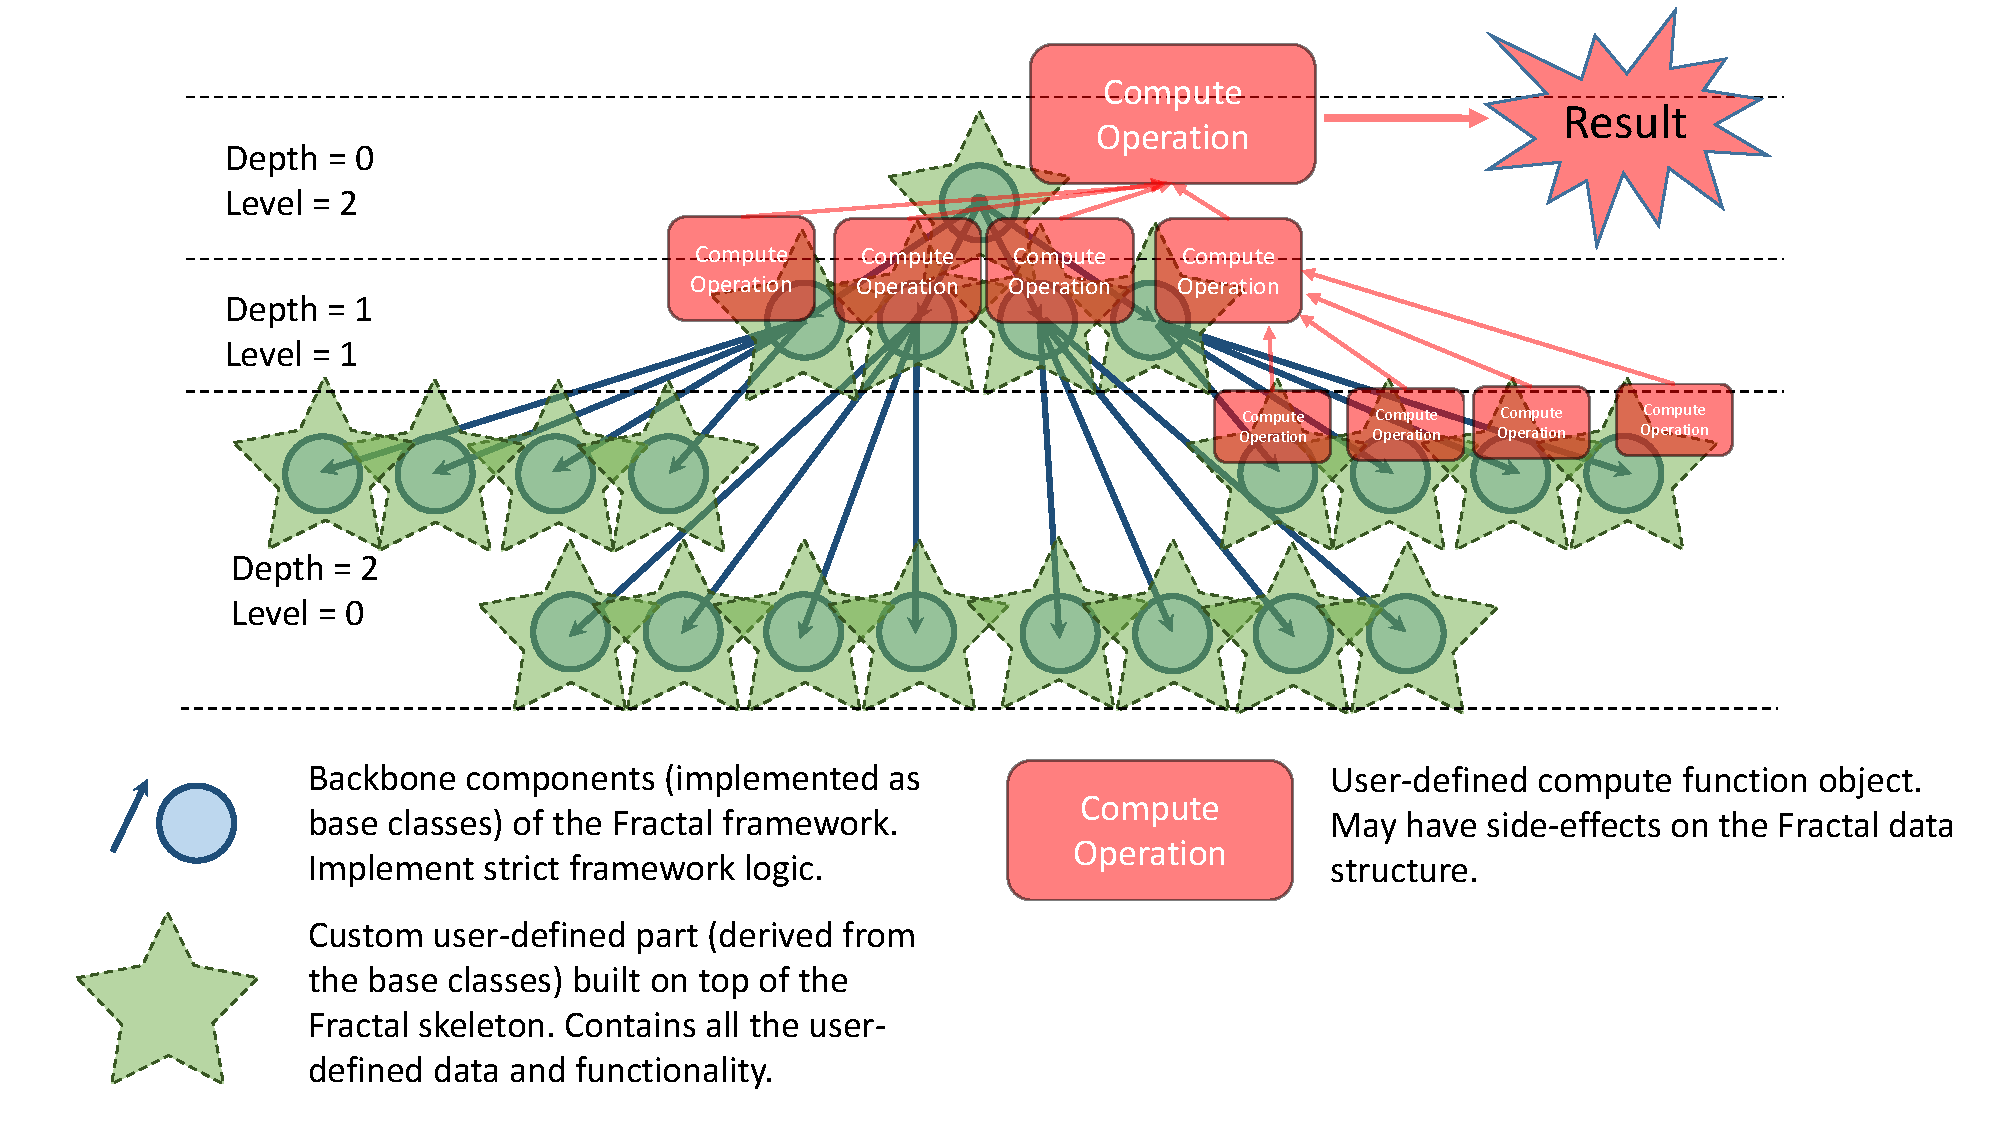
\includegraphics[width=1.0\textwidth]{images/Fractal.pdf}
\caption{The Fractal computational framework.}
\label{fig:fractal}
\end{figure}
\quad A more complicated and interesting fractal example would be a square being continuously and recursively divided into 4 equal sub-squares (southwest, northwest, southeast and northeast). The deep-growing structure is actually a 4-ary tree as well. Imagine one wants to compute the perimeter of some figure. One way to do it would be to map the figure on the square plane and then turn the plane into a grid by continuously splitting the square into 4 equal sub-parts (southwest, northwest, southeast, northeast) till we reach the granularity size of the grid. Then we paint all the grid elements located inside the figure shape as black and those outside of it as white. We iterate over the grid and detect all points of color flips and add the size of the grid elements to the final sum, which at the end is going to approximate the perimeter of the figure. That is roughly what the perimeter benchmark does.\newline\null
\quad In all its generality the fractal is a pattern, which can be characterized with self-similarity, repeatedness, structuredness, inherent parallelizability and the exact numeric values such as its depth and arity. All that naturally maps onto the C++ implementation as a class template we describe below.


\subsection{Fold}
\label{computational_frameworks_fold}
\quad The Fold computational framework has been inspired by the computation done in the power benchmark. The fold is not a new concept and has found a wide application in many functional languages. The C++ language provides std::accumulate() function template as a component of its Standard Template Library, which performs a functional fold over a given data structure, but contrary to our computational framework does not allow any side-effects and modifications to the elements of the data structure. Moreover, our C++ class template library provides an alternative interface to a user with an extensible customization space.\newline\null
\begin{figure}[ht]
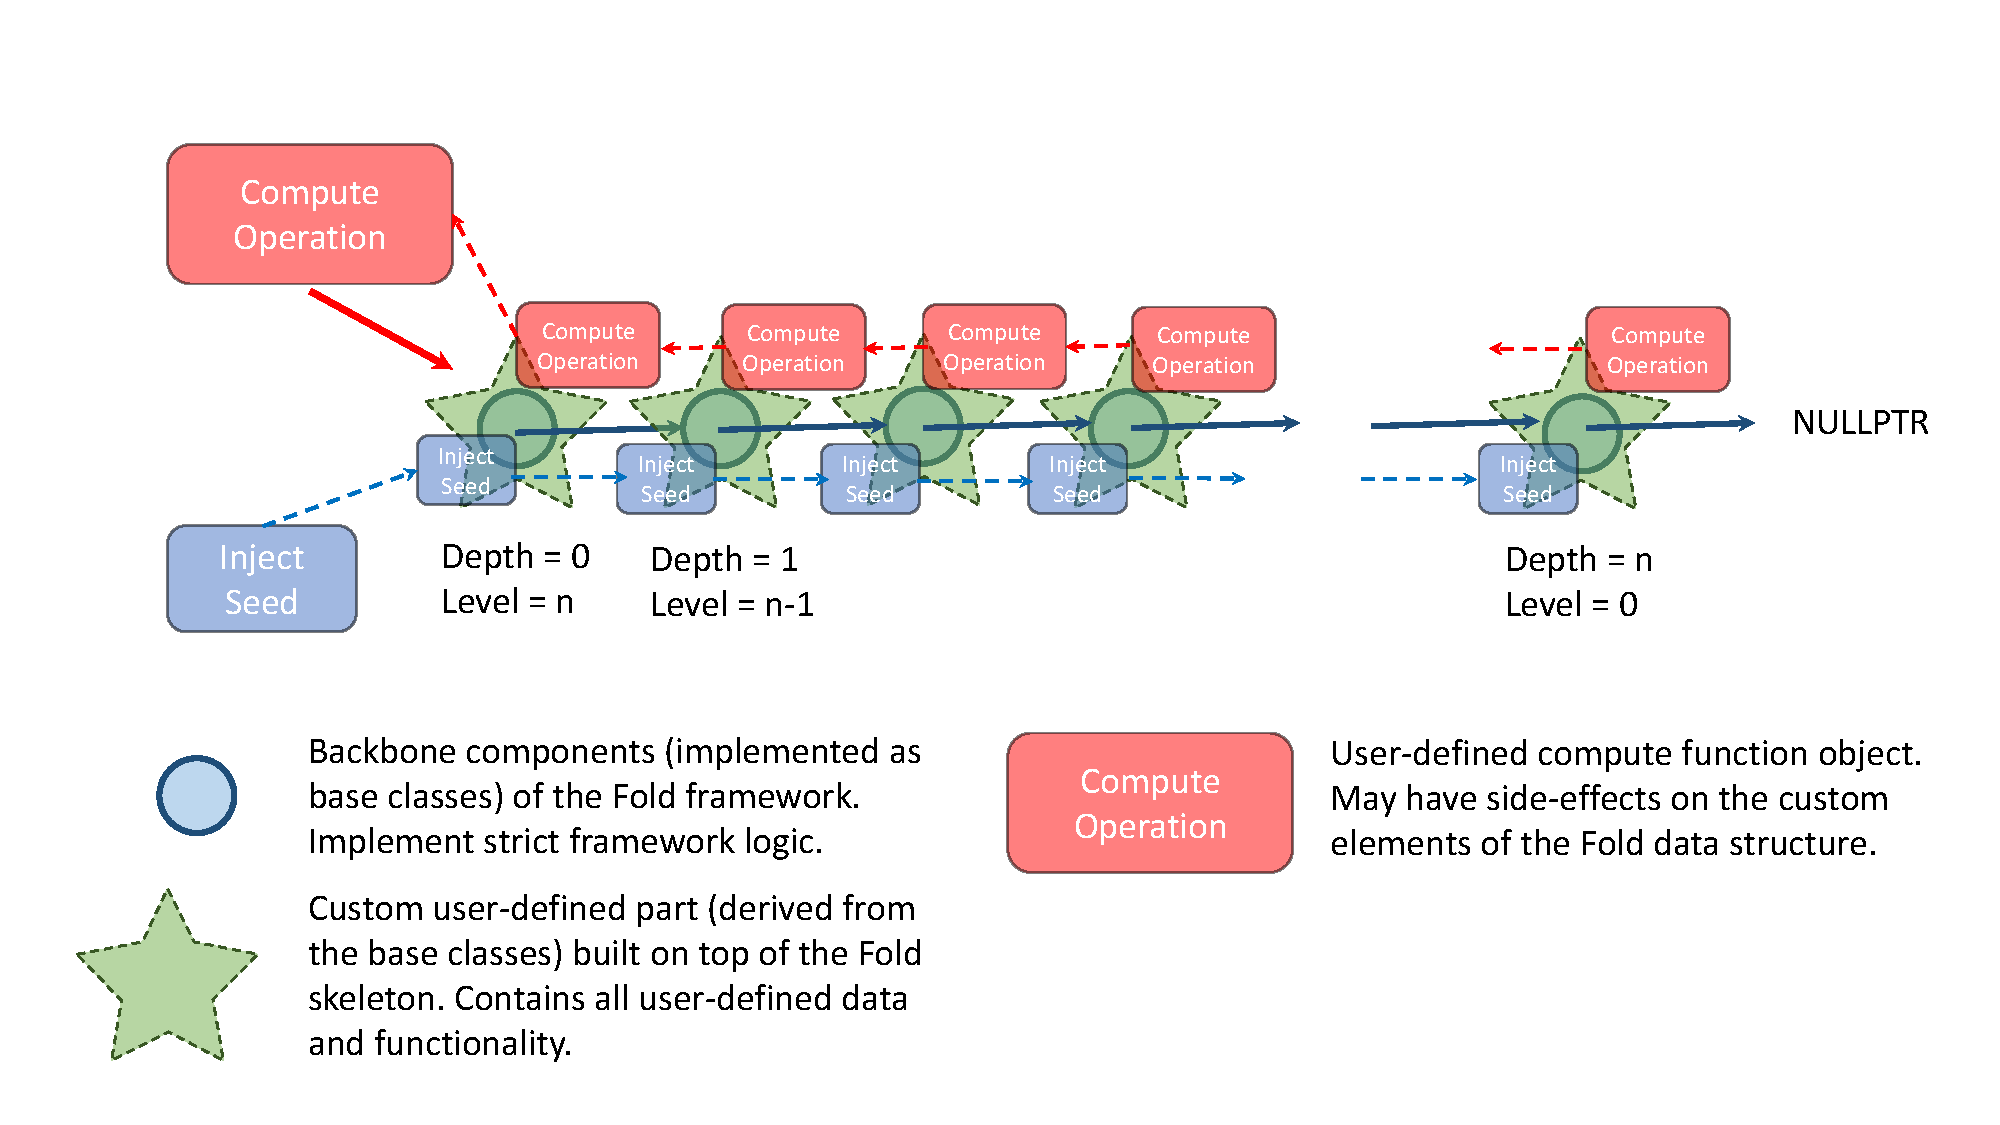
\includegraphics[width=1.0\textwidth]{images/Fold.pdf}
\caption{The Fold computational framework.}
\label{fig:fractal}
\end{figure}
\quad One can think of a Fold as a set of elements arranged into a linked-list. We grow the list to the specified depth given a seed value. Then we may inject some data into the head of the list and propagate it to its tail element. All propagation modifications are user-defined. Once every element of the list is ready with its data, the computation starts at the tail element and passes computed values back to previous elements of the chain.         


\subsection{Reduce}
\label{computational_frameworks_reduce}
\quad The Reduce computational framework is a well-known one. The difference between our computational framework and std::reduce() from C++ Standard Template Library (STL) is the possibility of having side effects and an alternative user customization interface. Our computational framework takes a function object with two overloaded and overridden virtual operator() methods. One specifies how to reduce the value from a single element (possibly changing the element in the process) and the other one defines the way of combining all the reduced values into the final return value. Our framework implements sequential as well as parallel Reduce versions.  


\subsection{Frameworks Library Design and Implementation}
\label{computational_frameworks_library_design}
\quad The design and implementation of computational frameworks library have been done iteratively using 4 Olden benchmarks as inspiration and  
The design of the C++ computational frameworks library aims at several goals.  
\begin{description}
\item[Modern C++] The implementation of the library is based on the Standard Template Library (STL) data structures, uses move semantics and unique pointers to achieve efficiency and smart memory management. For parallelization library uses OpenMP standard. All that provides for a wide source-code portability. The library is composed of a set of header files with class templates, which are supposed to be included into the user application.  
\item[Convenience] 
\item[Coherence] All computational frameworks in the library share the same user interface as well as internal design. Frameworks are inter-operable and flexible: one can create say, a fold of fractals of reductions. Different components can compute different return types.

\item[Sound design] CRTP, Algorithm Template pattern
\end{description}
\quad The computational frameworks are designed as a set of C++ class templates. The user interface these templates provide has been designed and refined iteratively using the set of Olden benchmarks [].     

\begin{minipage}[t]{\linewidth}
\begin{lstlisting}[caption={Computational framework class template skeleton},label={lst:framework_template_skeleton},language=C++]

template <typename ElemType, typename SeedType>
class Framework {
    public:
        class Element {
            // user-exposed customization iface
            virtual void grow(SeedType) = 0;
            virtual bool growth_stop_condition() { return false; }
        };
        template <typename ComputeType>
        class ComputeFunction {
            // framework specific application function API
            virtual operator()(ElemType& elem, ... ) = 0;
            virtual operator(const std::vector<ComputeType>&) = 0;
*       };
   /     
        void grow(size_t size, SeedType seed) {
            // organise framework elements 
            // into a data structure
            ... = new ElemType(); 
        }
        template<typename ComputeType>
        ComputeType compute(ComputeFunction<ComputeType>& apply_func);
    
    private:
        // framework data structure organisation
        // (list, tree, array, etc.)
};

\end{lstlisting}
\end{minipage}

\quad The design and the implementation of our template library reflect the target goals of the concept of computational frameworks.    

\quad There were several questions raised in the design process of a template library. 

\section{Performance study of the library}
\label{frameworks_performance_study}
\quad We have conducted a thorough performance examination of our prototype library. For that purpose we used 4 Olden benchmarks we are interested in. Benchmarks \textit{health}, \textit{treeadd} and \textit{perimeter} fit into our \textbf{fractal} framework and stress it from different angles. We used the \textit{power} benchmark to test the practical operation of our \textbf{fold} and \textbf{reduce} frameworks. We have rewritten the original sequential legacy C implementations of the benchmarks with our prototype library in a modern, structured and well-designed way. Thus, rejuvenating the code and parallelizing it in a well-structured and systematic manner. On the opposite side, these benchmarks inspired the concept of computational frameworks and shaped the design of the library.\newline\null 
\quad Performance plots below (figures \ref{fig:performance_health}, \ref{fig:performance_power_reduction_width}, \ref{fig:performance_treeadd}, \ref{fig:performance_perimeter}) show the strengths of the library, as well as its equally important weaknesses. The latter characterize applicability of the library, rather than the problems of the idea. In some places weaknesses highlight implementation problems, which are a matter of software engineering and not that of a research. The implementation can be easily configured to to be sequential or parallel, thus making it easy to conduct measurement experiments. Moreover, the fractal framework has 2 implementations under the hood. In the most general case the fractal is based on N-ary unbalanced tree. In this case we allocate it dynamically and every node has an array of pointers to its children. But in the case of a perfect (all leaves are at the same depth and every non-leaf node has all children present) tree, we can allocate all nodes linearly in an array-based heap manner. In the latter case parallelization happens per level, spawning the number of threads equal to the number of nodes at the given depth (provided that enough CPU cores are available). In the general case though we do not know where the growth of the fractal is going to stop and cannot index nodes on the array. Parallelization in the case of unbalanced fractal happens per child: spawning the number of threads equal to the number of children (again, provided that enough CPU cores are available). Figure \ref{fig:balanced_vs_unbalanced} illustrates two implementation strategies and performance plots below compare them.
\begin{figure}[!htb]
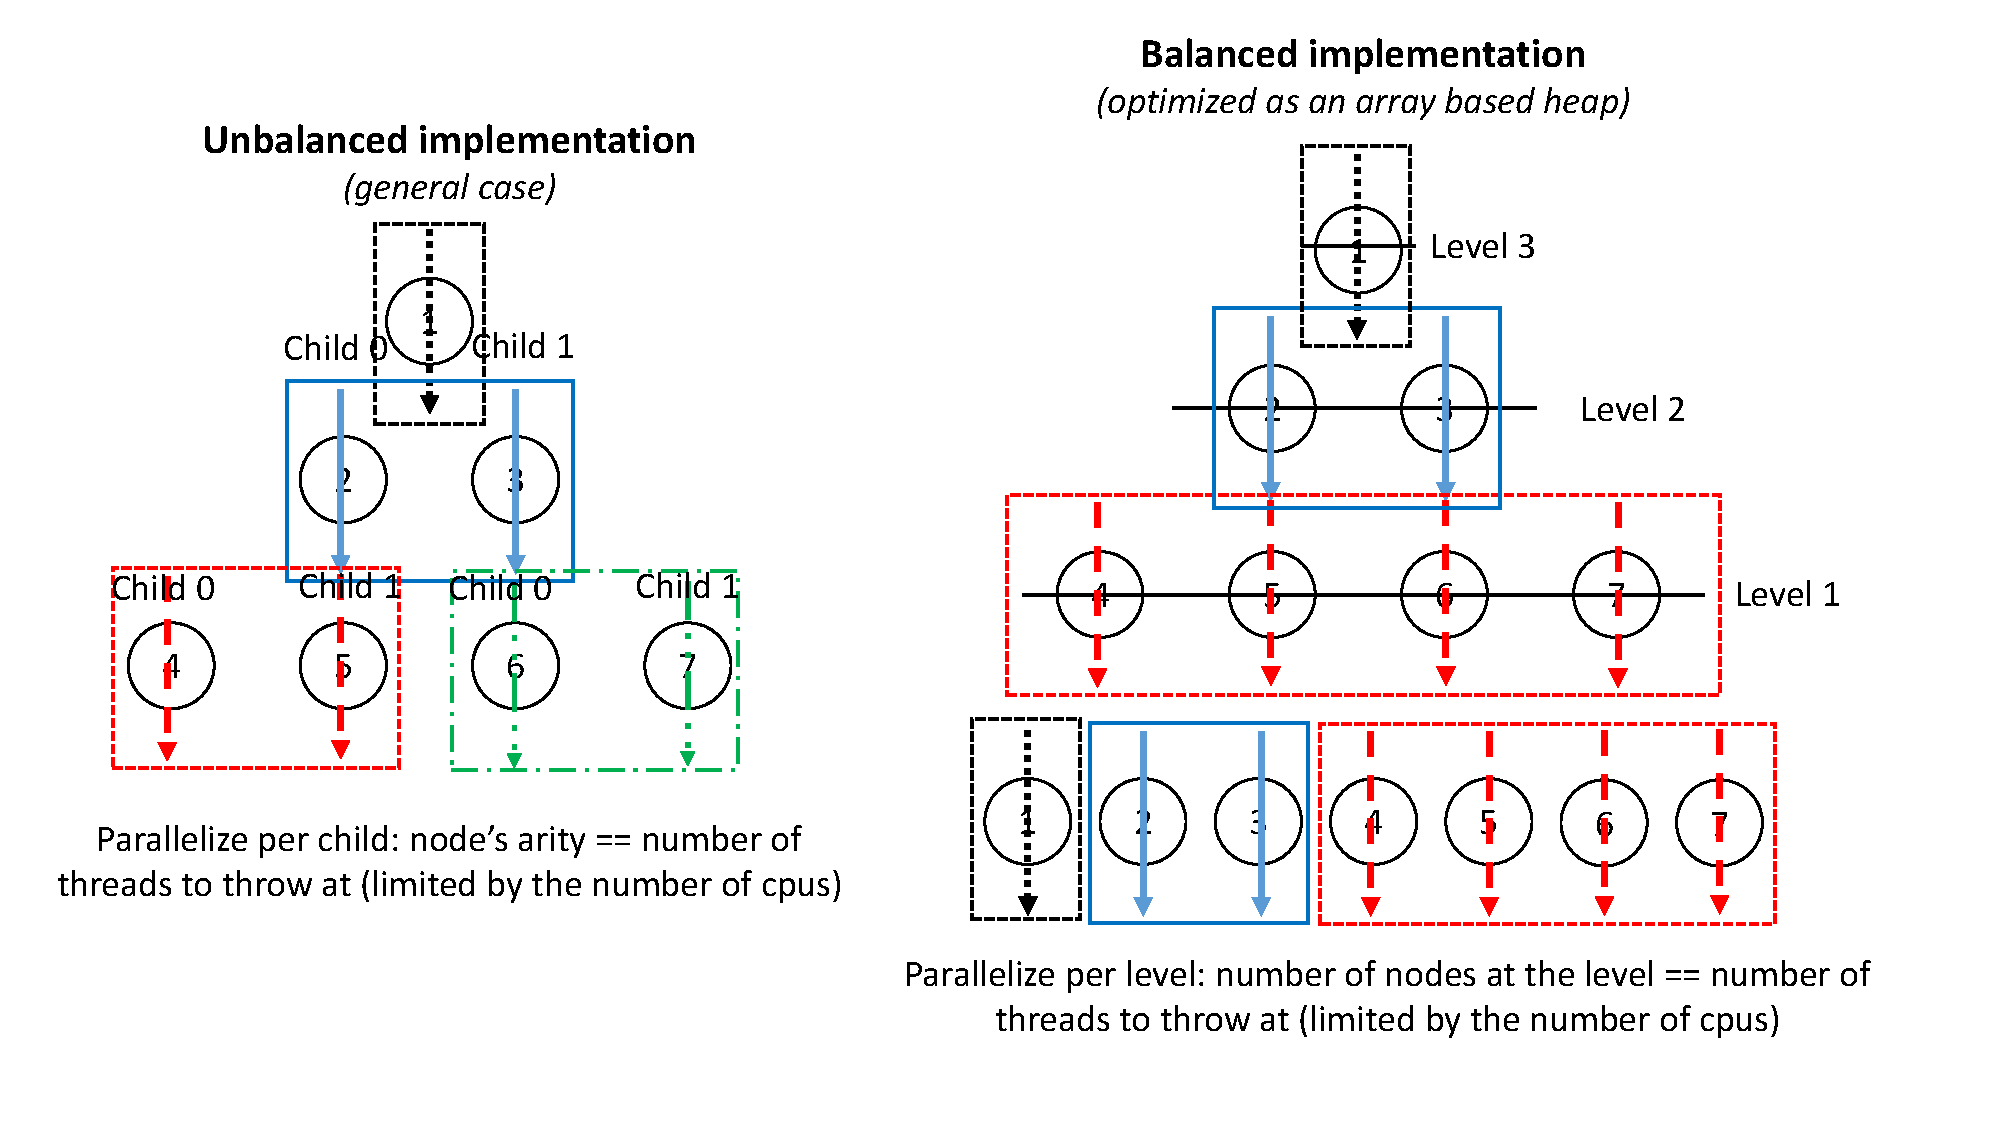
\includegraphics[width=1.0\textwidth]{images/balanced_vs_unbalanced.pdf}
\caption{\textit{Balanced} vs. \textit{Unbalanced} implementations of the fractal framework. Unbalanced implementation handles arbitrary tree and thus is based on pointers. Balanced implementation optimizes the case of a perfect tree and can be implemented with an array.}
\label{fig:balanced_vs_unbalanced}
\end{figure}\newline\null
\quad Figure \ref{fig:performance_health} demonstrates performance of various versions of the \textit{health} benchmark. The benchmark was described in section \ref{background_benchmarks_olden}. The benchmark grows a tree of hospitals and performs a simulation of the Columbian healthcare system step by step. The number of simulation steps done is plotted on the horizontal axis. The time a simulation took is plotted on a vertical axis. Nodes of the tree, which represent hospitals grow various lists of patients. As simulation goes the lists grow and the nodes become heavier. In other words, the state of the benchmark becomes bigger. The latter has an accumulating effect and contributes to the workload. We can see this phenomenon reflected in an exponential time growth of the sequential version. Parallel versions diminish this exponential time growth by tackling the task with several threads. This results into 5-6x speedups of the parallel versions relative to sequential ones. This benchmark is an ideal one to tackle with our fractal framework. And indeed, as figure \ref{fig:performance_health} shows, the thick lines representing the real time (wall clock time) indicate that a parallel version is consistently outperforming sequential version. The sequential versions of our library perform roughly as good as the original legacy C implementation (thin lines vs. a thick \textit{original} line). The latter shows that our library does not introduce any overheads on a benchmark with a significant workload.
\begin{figure}[!htb]
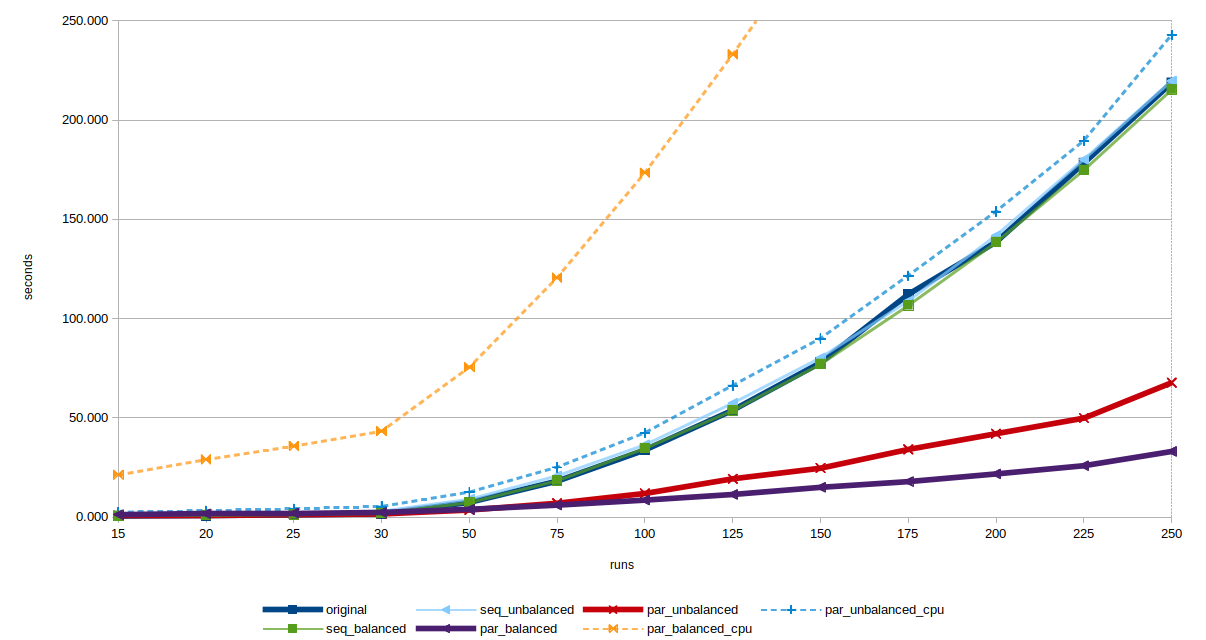
\includegraphics[width=1.0\textwidth]{images/health_depth_10.png}
\caption{Library performance on the \textit{health} benchmark. The legacy C implementation is represented by a thick \textit{original} line. Implementations of the benchmark based on our library are represented by 2 thick (\textit{parallel balanced} and \textit{unbalanced}) and 2 thin (\textit{sequential balanced} and \textit{unbalanced}) lines. Dotted lines represent the CPU time, which is not the real time and has a secondary importance. CPU time reflects the computational workload as we throw several threads at a task and can be used to judge on parallelization aggressiveness.}
\label{fig:performance_health}
\end{figure}\newline\null
\quad Figure \ref{fig:performance_power_reduction_width} illustrates the results for the \textit{power} benchmark. The benchmark performs a workload of scientific computations. The pattern is basically a reduction of folds of folds of reductions. So, the benchmark tests our \textbf{fold} and \textbf{reduce} frameworks. We can vary the width of reductions as well as the depth of folds to get various amounts of workload. The benchmark runs repeatedly until the computation result falls withing the set epsilon error. Figure \ref{fig:performance_power_reduction_width} illustrates how the running time of the benchmark scales with an increasing top level reduction width. The latter increases the workload and one can see the growing running time of the sequential original legacy C version. The sequential version based on our library runs roughly as good as the original one, while the parallel version is consistently outperforming both sequential versions. Dotted line again represents the CPU time and not the real time. CPU time approximately reflects how many threads were used to run the benchmark. As a validation, one can see that CPU time divided by parallel wall clock time is roughly corresponds to the reduction width. Behaviour of the \textit{power} benchmark is similar when we vary reduction widths or fold depths. For that reason we do not include the other experiments we ran.
\begin{figure}[!htb]
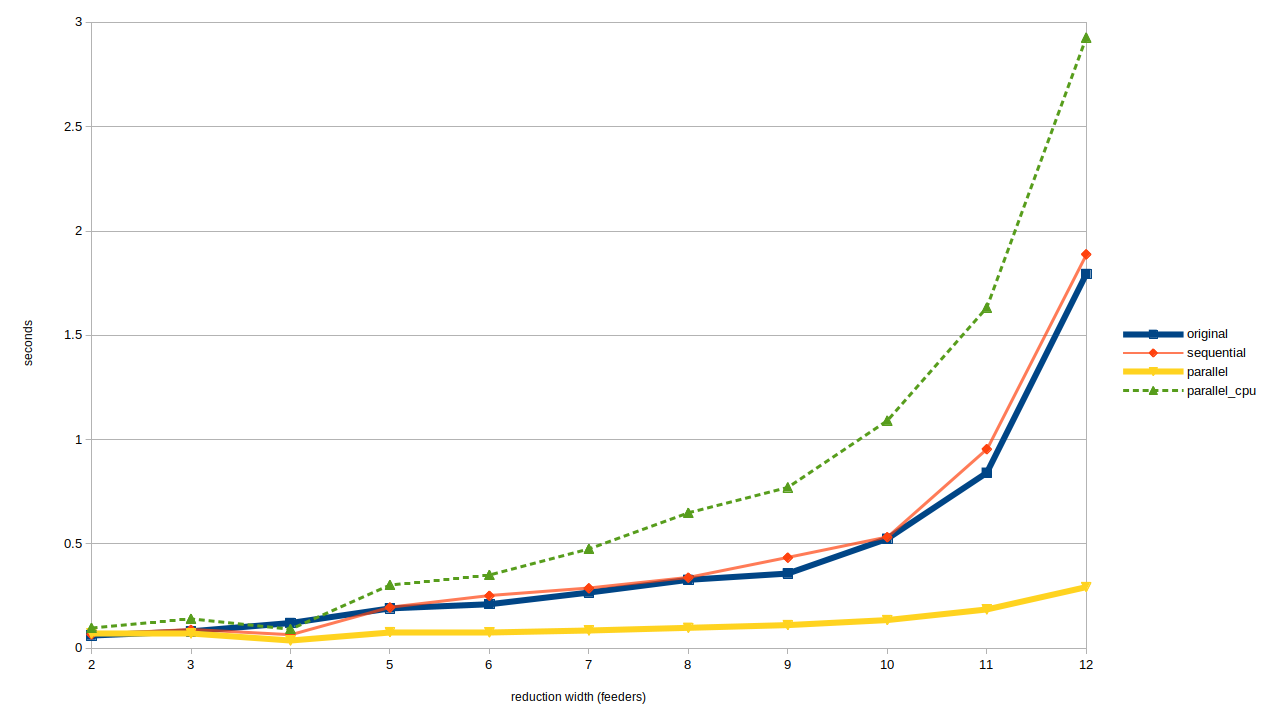
\includegraphics[width=1.0\textwidth]{images/power_reduction_width.png}
\caption{Library performance on the \textit{power} benchmark. We vary the top level (feeders) reduction width to scale the workload.}
\label{fig:performance_power_reduction_width}
\end{figure}\newline\null
\quad The \textit{health} and the \textit{power} benchmarks show the strengths of our library. The \textit{treeadd} and \textit{perimeter} benchmarks highlight its weaknesses. Figure \ref{fig:performance_treeadd} shows the behaviour of the \textit{treeadd} benchmark. This benchmark grows a tree with values at its nodes. Then it runs iteratively computing the reduction over the tree and updating node values. The computation is very lighweight and the state is minimal here. As we run the benchmark over and over the state does not grow. One can see a roughly linear running time of the original legacy C version. Overheads of our sequential library versions are striking for such a small benchmark, but again they can be optimized with a better engineered prototype library version and do not attribute to the research idea. The more threads we throw the bigger our overheads become. One can see it looking at the running time of balanced and unbalanced versions. It is worthless to tackle such a small benchmark with our library.      
\begin{figure}[!htb]
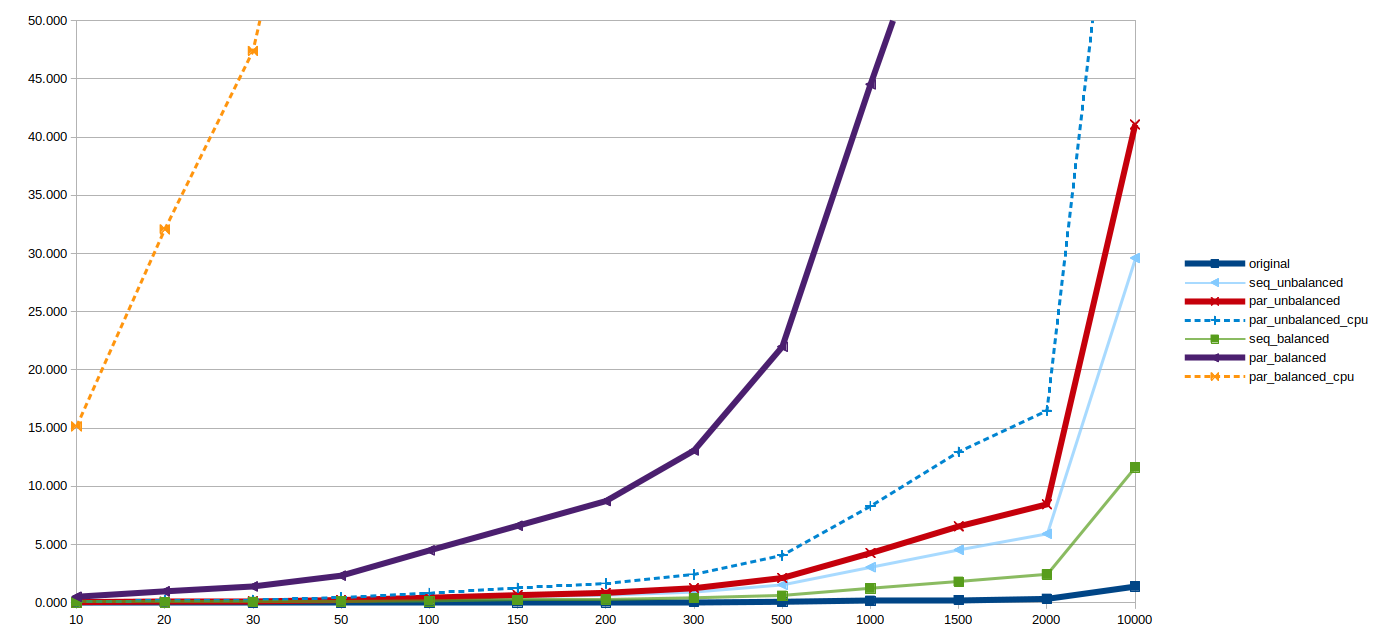
\includegraphics[width=1.0\textwidth]{images/treeadd_depth_16.png}
\caption{Library performance on the \textit{treeadd} benchmark.}
\label{fig:performance_treeadd}
\end{figure}\newline\null
\quad The \textit{perimeter} benchmark shows a different picture, but still highlights the current weaknesses of our prototype library implementation. Figure \ref{fig:performance_perimeter} shows the bar chart. As the benchmark is based on an unbalanced tree version we cannot run it with a balanced implementation. Here we have only the original sequential legacy C implementation, the sequential implementation based on our library and its parallel counterpart. One can see that the benchmark also highlights the current implementation problems: original does better than sequential. At the same time the benchmark has a potential: there is a good parallel speedup when we compare the sequential versus parallel library based versions. Although the library needs an optimization effort. Again, this is not the problem of an idea, but a mere software engineering task.
\begin{figure}[!htb]
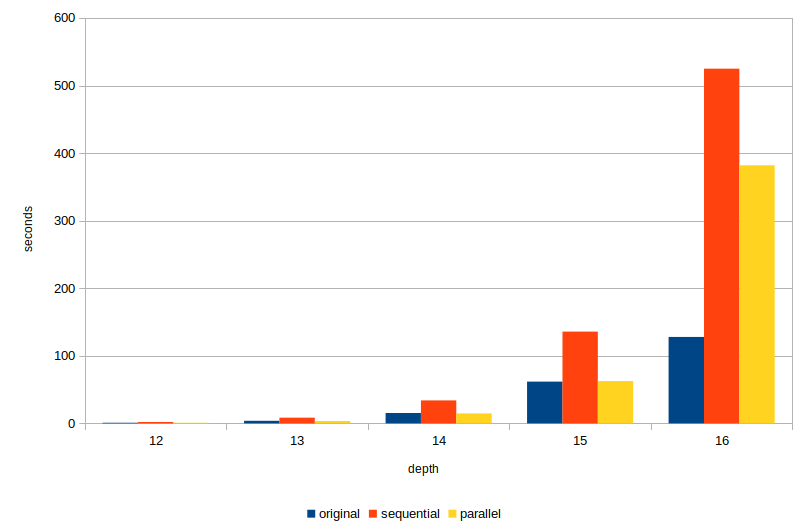
\includegraphics[width=1.0\textwidth]{images/perimeter.png}
\caption{Library performance on the \textit{perimeter} benchmark.}
\label{fig:performance_perimeter}
\end{figure}

\section{Future work}
\label{frameworks_future_work}
\quad The concept of computational frameworks and the prototype library form the basis for the future work. We believe that the process of software parallelization with the help of computational frameworks can be further automated for a relatively simple applications (like Olden benchmarks). Figure \ref{fig:parallelization_scheme} shows the scheme. It takes an original legacy C source code, where we supposedly have a computation that fits into one or several of our frameworks. The task of the recognizer is to identify a computational pattern. Like in the case of the \textit{health} Olden benchmark we have a recursive \textit{grow()} and \textit{compute()} procedures, which build and process the tree correspondingly. That recursive pattern can be matched to a fractal framework. The next step would be to strip the code corresponding and implementing the pattern (\textit{backbone logic}) and leave the rest as the \textit{business logic}. The business logic must be further classified into various computational framework template class methods (like \textit{grow()}, \textit{growth\_stop\_condition()}, \textit{inject()}, etc.). Then, the class template must be instantiated with the business logic inserted into the right places. Once that is done, the parallelization is done, as the compiler will take care of everything else.
\begin{figure}[!htb]
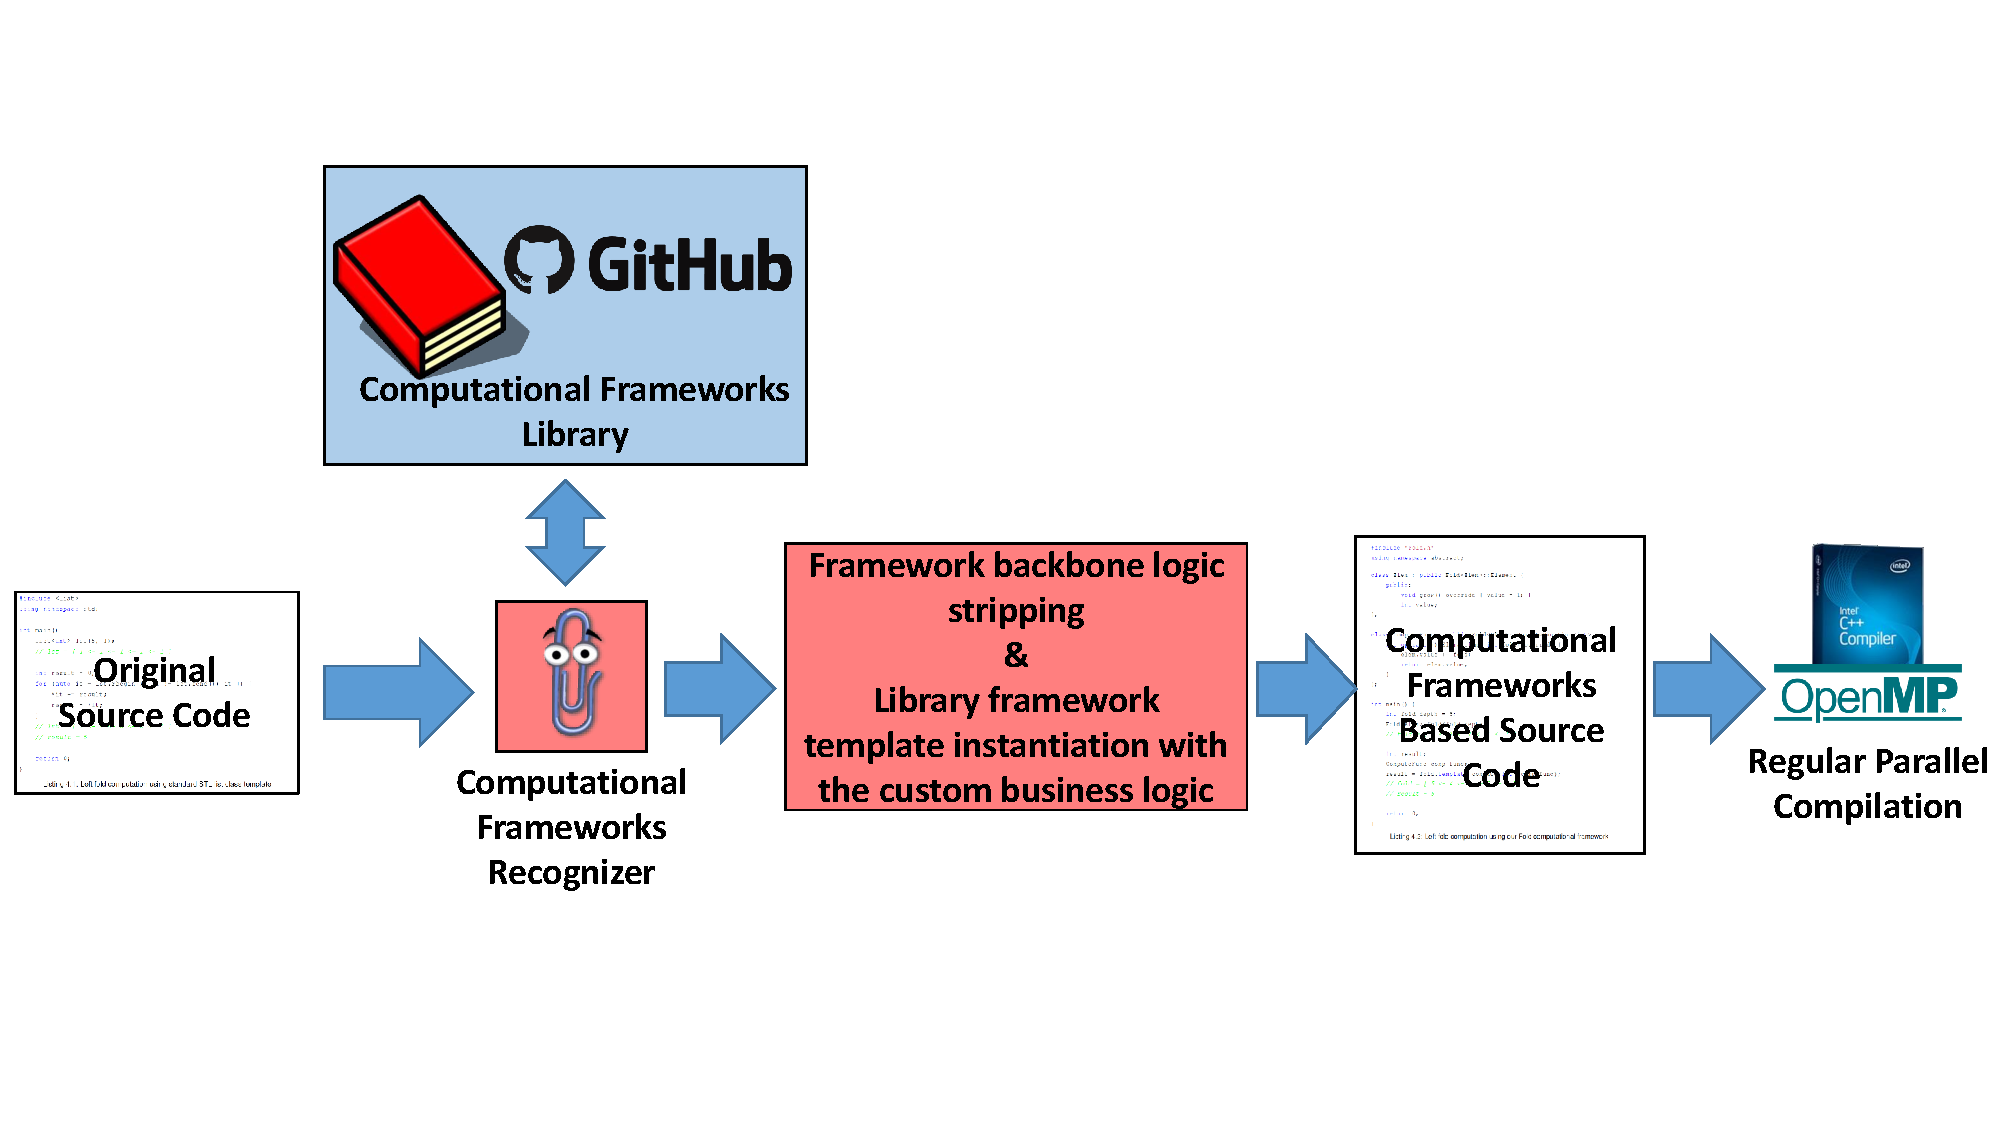
\includegraphics[width=1.0\textwidth]{images/parallelization_scheme.pdf}
\caption{An alternative software parallelization scheme based on our library of computational frameworks.}
\label{fig:parallelization_scheme}
\end{figure}\newline\null
\quad Technically, for benchmarks as simple as Olden the technique can work on the level of compiler's front end: source code or an abstract syntax tree (AST). That sets the technique apart from the regular parallelization approaches based on dependence graphs and working on the level of compiler's intermediate representation (IR).

%%